% Copyright (c) 2016 Benito Palacios Sánchez - All Rights Reserved.
% Esta obra está licenciada bajo la Licencia Creative Commons Atribución 4.0
% Internacional. Para ver una copia de esta licencia, visita
% http://creativecommons.org/licenses/by/4.0/.

% Template
\documentclass[usenames,dvipsnames]{beamer}
\pdfoutput=1

% Notes. Uncomment to view the notes.
%\setbeameroption{show notes}
%\setbeamertemplate{note page}[plain]    % Remove the note page style

% Load this package to allow load many big packages.
\usepackage{etex}

% Font
\usepackage[T1]{fontenc}        % Output font
\usepackage[utf8]{inputenc}     % Input encoding
\usepackage[spanish]{babel}     % For Spanish texts
\usepackage{FiraSans}           % For FiraSans beauty fonts

% Theme
\usetheme{Darmstadt}
\usecolortheme{whale}

% Other packages
\usepackage{xcolor}             % For color in text
\usepackage{url}                % For links
\usepackage{pifont}             % For tick symbol
\usepackage{graphicx}           % For graphics
\usepackage{epstopdf}           % For EPS graphics in Windows
\usepackage{multimedia}         % For media
\usepackage{ctable}             % For tables
\usepackage{verbatim}           % For non-parsed text blocks
\usepackage{tikz}               % To draw over images
\usepackage{textcomp}           % For text arrows.
\usepackage{listings}           % For blocks of code
\lstset{language=[Sharp]C,basicstyle=\scriptsize\ttfamily, keywordstyle=\scriptsize\color{blue}\ttfamily}

% My package
\usepackage{../Layout}

% Information about author and document
\title{Introducción al ROM Hacking}
\subtitle{Formatos comunes en juegos}
\date[Abril de 2016]{\today}
\author{Benito Palacios Sánchez}
\authortitle{}
\authoremail{benito.palaciossanchez.es@ieee.org}
\institute[IEEE SB UGR]{Rama estudiantil de IEEE en la UGR}
\titlelogo{../logo.png}

% Add a little logo in the corner of the slides
\pgfdeclareimage[height=0.5cm]{logo-mini}{../logo_mini.png}
\logo{\pgfuseimage{logo-mini}}

\begin{document}

    % Title page
    {
    \usebackgroundtemplate{
        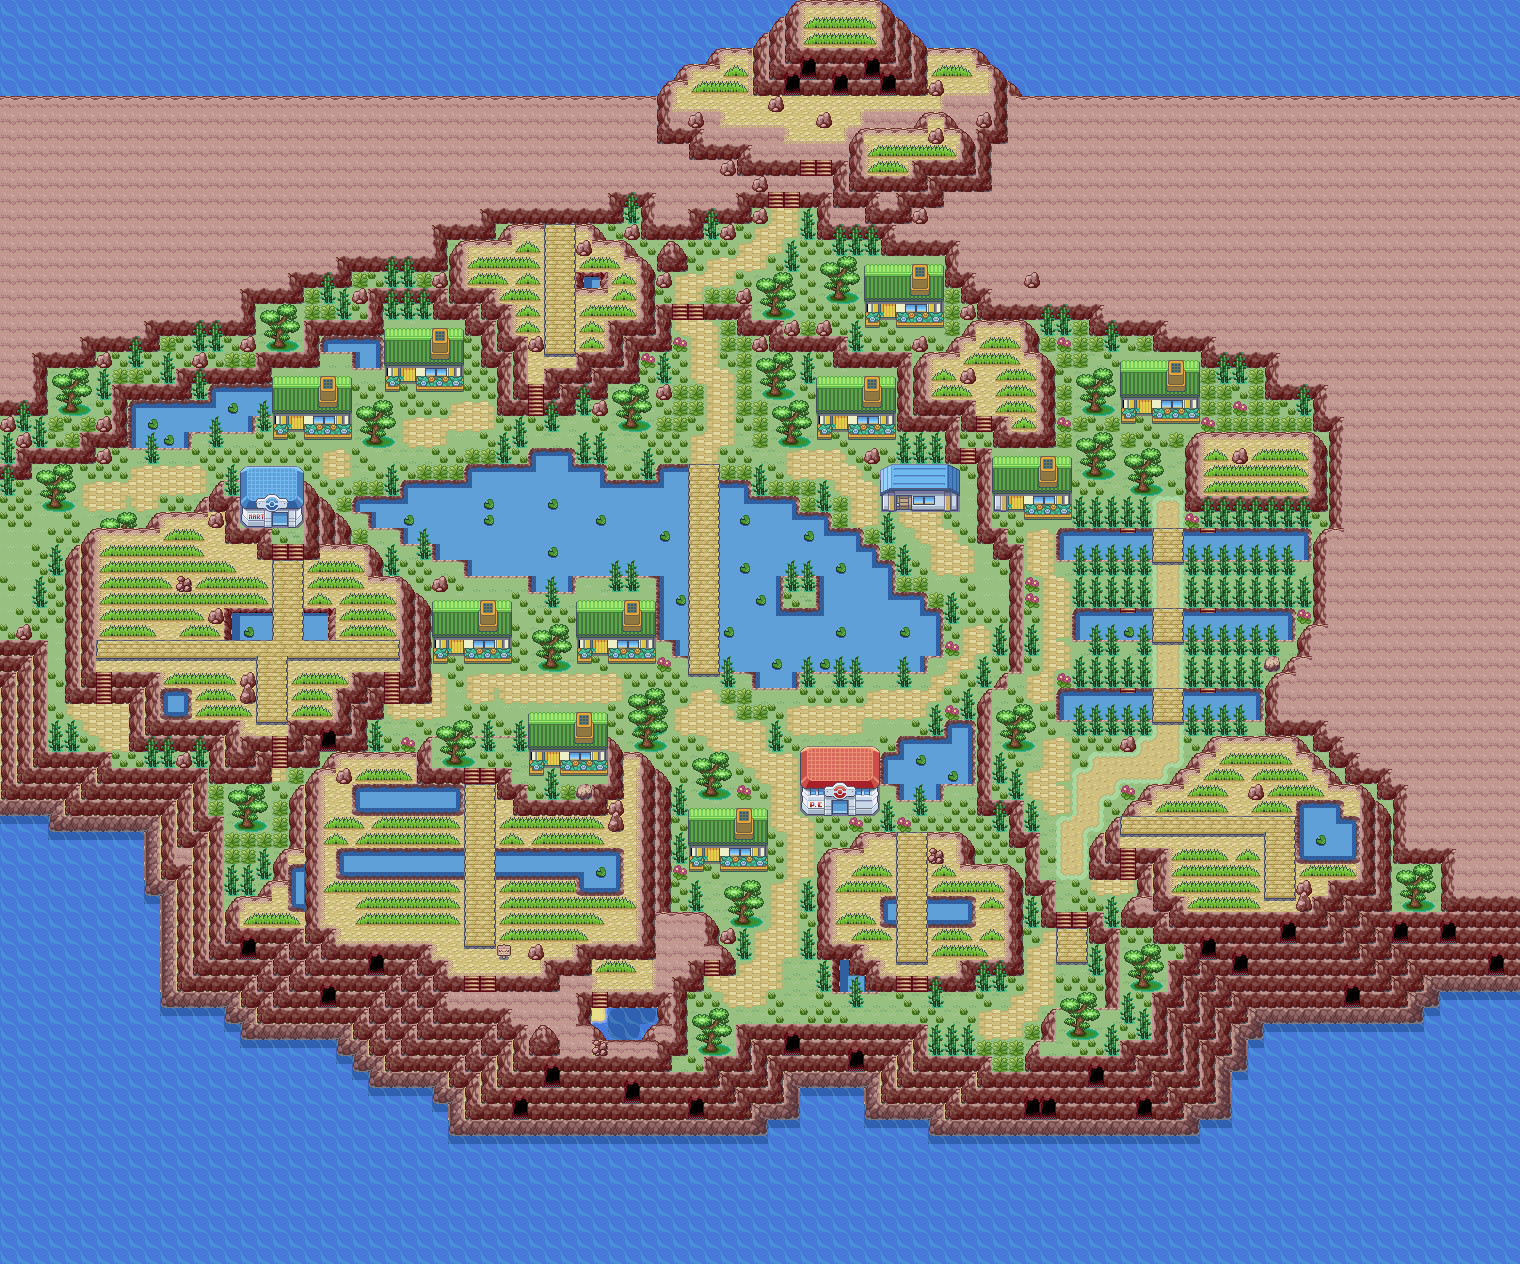
\includegraphics[width=\paperwidth]{../lesson1/imgs/bg_hack.jpg}}
    \begin{frame}[plain]
        \titlepage{}
    \end{frame}
    }

    % Content
    \begin{frame}{Contenido}
    \begin{columns}
    \begin{column}{0.5\textwidth}
        \uncover<2->{\large Textos}
        \begin{itemize}
            \item<2-> Codificaciones
            \item<2-> Formatos
        \end{itemize}
        \uncover<2->{Tipografías}
        \visible<2->{\includegraphics[width=0.8\textwidth]{imgs/example_text.png}}
    \end{column}
    \hfill
    \begin{column}{0.5\textwidth}
        \uncover<3->{\large Imágenes}
        \begin{itemize}
            \item<3-> Fondos
            \item<3-> Sprites
            \item<3-> Texturas
        \end{itemize}
        \vfill{}
        \visible<3->{\includegraphics[width=0.8\textwidth]{imgs/example_img.png}}
    \end{column}
    \end{columns}
\end{frame}

\section{Textos}
\begin{frame}{Naturaleza de los textos}
    \centering\Large ¿Cómo guardamos texto de forma digital?
    \includegraphics[width=0.75\textwidth]{imgs/example_text.png}
\end{frame}

\subsection{Codificaciones}
\begin{frame}{Codificación de caracteres}
    \centering
    \only<1>{
        \begin{block}{}
            Es el método que permite convertir un carácter de un lenguaje natural en un símbolo de otro sistema de representación aplicando reglas de codificación. [Wikipedia]
        \end{block}
    }
    \only<2>{\includegraphics[width=\textwidth]{imgs/ascii-table.png}}
\end{frame}

\begin{frame}{ASCII}
    \begin{block}{}
        \centering Codifica caracteres del alfabeto latino en 7 bits.
    \end{block}
    \begin{columns}
    \begin{column}{0.40\textwidth}
        \includegraphics[trim={1616px 0 0 0},clip,width=\textwidth]{imgs/ascii-table.png}
    \end{column}
    \begin{column}{0.55\textwidth}
        \centering
        \includegraphics[width=\textwidth]{imgs/text_hex.png} \\
        \Huge \textdownarrow \\
        \includegraphics[width=0.7\textwidth]{imgs/text_hex1.png}
    \end{column}
    \end{columns}
\end{frame}

\begin{frame}{Latin-1 (ISO 8859-1)}
    \begin{block}{}
        Codificación extendida de ASCII. Utiliza 8 bits añadiendo 128 caracteres necesarios para las lenguas europeas.
    \end{block}
    \centering\includegraphics[width=0.75\textwidth]{imgs/latin1.png}
\end{frame}

\begin{frame}{Unicode}
    \begin{block}{}
        Estándar universal de codificación de caracteres para la mayoría de lenguas (incluidas las muertas). La última version 6.0 incluye 109.449 caracteres.
    \end{block}

    \begin{itemize}
        \item<2-> Unicode es solo una tabla, no especifica la codificación.
        \item<3-> Codificaciones para unicode:
        \begin{itemize}
            \item<4-> UTF-8: codificación de 8 bits de longitud variable.\\ \texttt{'A' = 41h, '}\visible<4->{\includegraphics[height=7px]{imgs/rare_char.png}}\texttt{' = F0 A0 9C 8E}
            \item<5-> UTF-16: codificación de 16 bits de longitud variable. \\ \texttt{'A' = 0041, '}\visible<5->{\includegraphics[height=7px]{imgs/rare_char.png}}\texttt{' = D841 DF0E}
            \item<6-> UTF-32: codificación de 8 bits de longitud fija. \\ \texttt{'A' = 00000041, '}\visible<6->{\includegraphics[height=7px]{imgs/rare_char.png}}\texttt{' = 0002070E}
        \end{itemize}
    \end{itemize}
\end{frame}

\begin{frame}{Shift Jis (CP 932)}
    \begin{block}{}
        Codificación de longitud variable (1 o 2 bytes) para caracteres japoneses. Incluye ASCII.
    \end{block}
    \includefigure{Tabla para caracteres con primer byte \texttt{0x82}}{imgs/shiftjis_table82.png}{0.55}
\end{frame}

\begin{frame}{Ejemplos en archivos}
    \centering\Large
    \only<1>{¿? \\}
    \only<2->{UTF-16 \\}
    \includegraphics[width=0.75\textwidth]{imgs/utf16.png} \\
    \only<3>{¿? \\}
    \only<4->{Shift Jis \\}
    \visible<3->{\includegraphics[width=0.75\textwidth]{imgs/shiftjis.png}}
\end{frame}

\begin{frame}{Tablas}
    Algunos juegos usan codificaciones propietarias...
    \begin{itemize}
        \item ... fácil \textit{mapeo} con la tipografía.
        \item ... dificultar el acceso.
    \end{itemize}
    \includefigure{Textos de Pokémon Perla}{imgs/text_perla.png}{1}
\end{frame}

\begin{frame}[t,fragile]{Tablas}
    \includegraphics[width=\textwidth]{imgs/text_perla_trans.png}
    \footnotesize\ctable[]{cc|cc|cc}{}{                                     \FL
Valor          & Caracter & Valor          & Caracter & Valor    & Caracter \ML
\texttt{01A9h} & ¡        & \texttt{01ABh} & !        & \texttt{01ADh} & ,  \NN
\texttt{01DEh} & \textit{SP} & \texttt{E000h} & \textit{NL} & \texttt{0152h} & E \NN
\texttt{0132h} & H        & \texttt{013Ah} & P        & \texttt{013Eh} & T  \NN
\texttt{0145h} & a        & \texttt{0147h} & c        & \texttt{0148h} & d  \NN
\texttt{014Ch} & h        & \texttt{0150h} & l        & \texttt{0152h} & n  \NN
\texttt{0153h} & o        & \texttt{0156h} & r        & \texttt{0158h} & t  \LL
    }
\end{frame}

\subsection{Formatos}
\begin{frame}{Punteros (\textit{offsets})}
    \begin{block}{}
        \centering{}Número enteros que indican la posición del texto.
    \end{block}
    \vfill{}
    \uncover<2->{\large Tipos:}
    \begin{itemize}
        \item<3-> \textit{Absoluto}: desde el comienzo del archivo.
        \item<4-> Relativo: desde otra posición
        \begin{itemize}
            \item Relativo a una sección del fichero.
            \item Relativo a la posición actual.
        \end{itemize}
    \end{itemize}
\end{frame}

\begin{frame}{Punteros (\textit{offsets})}
    \centering\Large Formato \texttt{BMG}
    \vfill{}
    \begin{tikzpicture}
        \node[anchor=south west,inner sep=0] (image) at (0,0)
        {\includegraphics[width=\textwidth]{imgs/pointers.png}};
            \begin{scope}[x={(image.south east)},y={(image.north west)}]
                \draw[black,thick] (0.775,0) -- (0.775,1);
                \draw<2-4>[red,semithick] (0.13,0.9) rectangle (1,0.57);
                \draw<2-4>[blue,semithick] (0.13,0.565) rectangle (1,0.0);
                \draw<3,4>[blue,semithick] (0.13,0.565) rectangle (0.446,0.495);
                \draw<4->[blue,line width=2pt,->] (0.446,0.65) -- (0.446,0.55);
                \draw<5,6>[red,semithick] (0.13,0.81) rectangle (0.29,0.745);
                \draw<6>[blue,semithick] (0.765,0.565) -- (0.53,0.565) -- (0.53,0.495) -- (0.765,0.495);
                \draw<6>[blue,semithick] (1,0.565) -- (0.913,0.565) -- (0.913,0.495) -- (1,0.495);
                \draw<6>[blue,semithick] (0.78,0.49) -- (0.835,0.49) -- (0.835,0.41) -- (0.78,0.41);
                \draw<6>[blue,semithick] (0.13,0.49) -- (0.29,0.49) -- (0.29,0.41) -- (0.13,0.41);
                \draw<7,8>[red,semithick] (0.45,0.81) rectangle (0.60,0.745);
                \draw<8,9>[blue,semithick] (0.13, 0) -- (0.13, 0.4) -- (0.29, 0.4) -- (0.29,0.49) -- (0.765, 0.49) -- (0.765, 0);
                \draw<8,9>[blue,semithick] (0.78, 0) -- (0.78, 0.4) -- (0.835, 0.4) -- (0.835, 0.49) -- (1, 0.49) -- (1, 0);
                \draw<9>[green,semithick] (0.21, 0.49) rectangle (0.29, 0.4);
                \draw<9>[green,semithick] (0.37, 0.4) rectangle (0.445, 0.32);
                \draw<9>[green,semithick] (0.37, 0.24) rectangle (0.445, 0.16);
            \end{scope}
    \end{tikzpicture}
\end{frame}

\section{Imágenes}
\begin{frame}{Naturaleza de las imágenes}
    \centering\Large ¿Qué necesitamos para formar una imagen?
    \includegraphics[width=0.75\textwidth]{imgs/example_img.png}
\end{frame}

\subsection{Imágenes de fondo}
\begin{frame}{Partes de una imagen}
    \begin{block}{}
        \centering{}Una imagen se compone de sucesión de colores (píxeles).
    \end{block}
    \vfill{}
    \begin{columns}
    \begin{column}{0.25\textwidth}
        \visible<2->{\includegraphics[width=\textwidth]{imgs/zelda_pal.png}}
    \end{column}
    \begin{column}{0.05\textwidth}
        \visible<3->{\huge +}
    \end{column}
    \begin{column}{0.5\textwidth}
        \visible<3->{\includegraphics[width=\textwidth]{imgs/zelda_px.png}}
    \end{column}
    \begin{column}{0.05\textwidth}
        \visible<4->{\huge =}
    \end{column}
    \begin{column}{0.25\textwidth}
        \visible<4->{\includegraphics[width=\textwidth]{imgs/example_img.png}}
    \end{column}
    \end{columns}
\end{frame}

\begin{frame}{Colores}
    \begin{block}{}
        Los colores se forman \textit{mezclando} los tres colores base (componentes / canal): \textbf{rojo}, \textbf{verde} y \textbf{azul}.
    \end{block}
    \begin{columns}
    \begin{column}{0.2\textwidth}
        \centering
        \includegraphics[width=\textwidth]{imgs/rgb.png}
    \end{column}
    \begin{column}{0.8\textwidth}
        \small
        \begin{itemize}
            \item<2-> El rango de valores de cada componente define los colores únicos.
            \item<3-> Generalmente: 8 bits/canal \\
            $2^8=256\rightarrow 256^3=16.777.216$ colores únicos.
            \item<4-> NDS: 5 bits (\texttt{BGR555}) $\rightarrow$ 32.768 colores únicos.
            \begin{itemize}
                \item<4-> Un color ocupa 16 bits:\\
                5 por canal + 1 transparencia.
            \end{itemize}
        \end{itemize}
    \end{column}
    \end{columns}
\end{frame}

\begin{frame}{Paletas}
    \begin{block}{}
        Agrupación de colores. Definen los colores de una imagen. El primer color suele ser el transparente.
    \end{block}
    {\centering\includegraphics[width=0.25\textwidth]{imgs/zelda_pal.png}\\}
    \uncover<2->{Modalidades:}
    \begin{itemize}
        \item<2-> 1 paleta de 256 colores = 256 colores.
        \item<3-> 16 paletas de 16 colores = 256 colores.
        \item<4-> 16 paletas de 256 colores = 4.096 colores.
    \end{itemize}
\end{frame}

\begin{frame}{Píxeles}
    \begin{block}{}
        La información que guardamos por píxel es la posición en la paleta de su color.
    \end{block}
    {\centering\includegraphics[width=0.25\textwidth]{imgs/zelda_px.png}\\}
    \uncover<2->{Codificaciones:}
    \begin{itemize}
        \item<2-> 8 bits por píxel (bpp): $2^8=256$ posiciones diferentes $\rightarrow$ 256 colores diferentes.
        \item<3-> 4 bpp: 16 colores diferentes.
        \item<4-> 1 bpp: 2 colores diferentes (blanco o negro).
    \end{itemize}
\end{frame}

\begin{frame}{Agrupación de píxeles}
    \centering
    \only<1,3>{
    \begin{tikzpicture}
        \node[anchor=south west,inner sep=0] (image) at (0,0)
        {\includegraphics[width=256px]{imgs/example_img.png}};
        \begin{scope}[x={(image.south east)},y={(image.north west)}]
            \draw<3>[help lines,xstep=8bp,ystep=8bp] (0,0) grid (1,1);
        \end{scope}
    \end{tikzpicture}
    }
    \only<2>{
    \includegraphics[width=\textwidth]{imgs/img_lineal.png}
    }
\end{frame}

\begin{frame}[fragile]{Agrupación de píxeles}
    \begin{columns}
    \begin{column}{0.1\textwidth}
        \begin{tikzpicture}
            \node[anchor=south west,inner sep=0] (image) at (0,0)
            {\includegraphics[width=16px]{imgs/small_img.png}};
            \begin{scope}[x={(image.south east)},y={(image.north west)}]
                \draw[help lines,xstep=8bp,ystep=8bp] (0,0) grid (1,1);
            \end{scope}
        \end{tikzpicture}
    \end{column}
    \begin{column}{0.9\textwidth}
        {\textbf{Lineal}}
        \begin{lstlisting}[basicstyle=\ttfamily\footnotesize]
00 01 02 03 04 05 06 07 08 09 0A 0B 0C 0D 0E 0F
10 11 12 13 14 15 16 17 18 19 1A 1B 1C 1D 1E 1F
20 21 22 23 24 25 26 27 28 29 2A 2B 2C 2D 2E 2F
30 31 32 33 34 35 36 37 38 39 3A 3B 3C 3D 3E 3F
40 41 42 43 44 45 46 47 48 49 4A 4B 4C 4D 4E 4F
        \end{lstlisting}
        \begin{uncoverenv}<2->{\textbf{Horizontal}}
        \begin{lstlisting}[basicstyle=\ttfamily\footnotesize\color{red},
            belowskip=-0.5\baselineskip]
00 01 02 03 04 05 06 07 10 11 12 13 14 15 16 17
20 21 22 23 24 25 26 27 30 31 32 33 34 35 36 37
40 41 42 43 44 45 46 47 50 51 52 53 54 55 56 57
60 61 62 63 64 65 66 67 70 71 72 73 74 75 76 77\end{lstlisting}
        \begin{lstlisting}[basicstyle=\ttfamily\footnotesize\color{blue}]
08 09 0A 0B 0C 0D 0E 0F 18 19 1A 1B 1C 1D 1E 1F
        \end{lstlisting}\end{uncoverenv}
    \end{column}
    \end{columns}
\end{frame}

\begin{frame}{Compresión}
    \only<1>{
    \centering
    \begin{tikzpicture}
        \node[anchor=south west,inner sep=0] (image) at (0,0)
        {\includegraphics[width=256px]{imgs/zelda_nintendo.png}};
        \begin{scope}[x={(image.south east)},y={(image.north west)}]
            \draw[help lines,xstep=8bp,ystep=8bp] (0,0) grid (1,1);
        \end{scope}
    \end{tikzpicture}
    }
    \only<2-4>{
    \centering
    \begin{columns}
    \begin{column}{0.15\textwidth}
        \begin{tikzpicture}
            \node[anchor=south west,inner sep=0] (image) at (0,0)
            {\includegraphics[width=48px]{imgs/zelda_nintendo_compress.png}};
            \begin{scope}[x={(image.south east)},y={(image.north west)}]
                \draw[help lines,xstep=8bp,ystep=8bp] (0,0) grid (1,1);
            \end{scope}
        \end{tikzpicture}
    \end{column}
    \begin{column}{0.05\textwidth}
        \visible<3->{\huge +}
    \end{column}
    \begin{column}{0.5\textwidth}
        \visible<3->{\includegraphics[width=\textwidth]{imgs/screen_info.png}}
    \end{column}
    \begin{column}{0.05\textwidth}
        \visible<4->{\huge =}
    \end{column}
    \begin{column}{0.25\textwidth}
        \visible<4->{\includegraphics[width=\textwidth]{imgs/zelda_nintendo.png}}
    \end{column}
    \end{columns}
    }
    \only<5-6>{
    \begin{columns}
    \begin{column}{0.5\textwidth}
        \centering
        \includegraphics[width=0.7\textwidth]{imgs/map_ninokuni_mess.png}
    \end{column}
    \begin{column}{0.05\textwidth}
        \visible<6->{\huge$\rightarrow$}
    \end{column}
    \begin{column}{0.5\textwidth}
        \centering
        \visible<6->{
        \includegraphics[width=0.7\textwidth]{imgs/map_ninokuni_fix1.png} \\
        \vspace{10pt}
        \includegraphics[width=0.7\textwidth]{imgs/map_ninokuni_fix2.png}
        }
    \end{column}
    \end{columns}
    }
    \only<7->{
    Compresión de \textit{tiles}:
    \begin{itemize}
        \item<7-> Evita guardar \textit{tiles} idénticos.
        \item<8-> Evita guardar \textit{tiles volteados} horizontalmente o verticalmente.
        \item<9-> Permite agrupar imágenes.
        \item<10-> Permite usar 256 colores distintos en formatos 4bpp.
        \begin{itemize}
            \item<11-> Cada \textit{tile} usa una paleta.
        \end{itemize}
    \end{itemize}
    }
\end{frame}

\subsection{Sprites}
\begin{frame}{Casos de uso}
    \only<1-4>{
    \begin{columns}
    \begin{column}{0.5\textwidth}
        \centering
        \textbf{Capas} \\ \vspace{10pt}
        \only<1>{\includegraphics[width=\textwidth]{imgs/zelda_title.png}}
        \only<2->{\includegraphics[width=\textwidth]{imgs/zelda_title_cells.png}}
    \end{column}
    \hfill
    \begin{column}{0.5\textwidth}
        \centering
        \uncover<3->{\textbf{Animaciones}} \\ \vspace{10pt}
        \visible<3->{\includegraphics[width=30px]{imgs/zelda_anm-0.png}}
        \visible<4>{
        \vfill{}
        \includegraphics[width=30px]{imgs/zelda_anm-1.png}\hfill{}
        \includegraphics[width=30px]{imgs/zelda_anm-2.png}\hfill{}
        \includegraphics[width=30px]{imgs/zelda_anm-3.png}
        }
    \end{column}
    \end{columns}
    }

    \only<5>{
    \centering
    \textbf{Ahorro de espacio con capas}
    \vfill{}
    \begin{columns}
    \begin{column}{0.25\textwidth}
        \includegraphics[width=\textwidth]{imgs/zelda_btn_base.png}
    \end{column}
    \begin{column}{0.05\textwidth}
        \huge +
    \end{column}
    \begin{column}{0.2\textwidth}
        \includegraphics[width=\textwidth]{imgs/zelda_btn_text1.png}
        \vspace{10pt}
        \includegraphics[width=\textwidth]{imgs/zelda_btn_text2.png}
    \end{column}
    \begin{column}{0.05\textwidth}
        \huge =
    \end{column}
    \begin{column}{0.25\textwidth}
        \includegraphics[width=\textwidth]{imgs/zelda_btn1.png}
        \vspace{10pt}
        \includegraphics[width=\textwidth]{imgs/zelda_btn2.png}
    \end{column}
    \end{columns}
    }
\end{frame}

\begin{frame}{Formatos base}
    \begin{columns}
    \begin{column}{0.45\textwidth}
        \centering{}Paleta \\ \vspace{5pt}
        \includegraphics[width=\textwidth]{imgs/zelda_title_pal.png}
    \end{column}
    \begin{column}{0.05\textwidth}
        \uncover<2>{\huge +}
    \end{column}
    \begin{column}{0.45\textwidth}
        \centering{}\uncover<2>{\textit{Tiles}} \\ \vspace{5pt}
        \visible<2>{\includegraphics[width=\textwidth]{imgs/zelda_title_px.png}}
    \end{column}
    \end{columns}
\end{frame}

\begin{frame}{Celdas}
    \centering{}Nitro CElls Resource (.ncer) \\ \vspace{5pt}
    \includegraphics[width=0.6\textwidth]{imgs/zelda_title_ui.png}
\end{frame}

\begin{frame}{Animaciones}
    \centering{}Nitro AnimatioN Resource (.nanr) \\ \vspace{5pt}
    \includegraphics[width=0.6\textwidth]{imgs/zelda_anm_ui.png}
\end{frame}

\subsection{3D}
\begin{frame}{Texturas}
    \centering{}Nitro TeXture (.nsbtx) \\ \vspace{5pt}
    \begin{columns}
    \begin{column}{0.5\textwidth}
        \only<1-3>{\includegraphics[width=\textwidth]{imgs/zelda_link_tex.png}}
        \only<4>{\includegraphics[width=\textwidth]{imgs/zelda_house_tex.png}}
    \end{column}
    \begin{column}{0.6\textwidth}
        \begin{wideitemize}
            \item<1-> Uso en modelos 3D
            \item<2-> Paletas + \textit{Tiles}
            \item<3-> Codificaciones: A3I5, A4I4, A5I3, 4x4 texel
        \end{wideitemize}
    \end{column}
    \end{columns}
\end{frame}

\begin{frame}{Modelos 3D}
    \begin{columns}
    \begin{column}{0.5\textwidth}
        \begin{wideitemize}
            \item<1-> Geometría 3D.
            \item<2-> Comandos de OpenGL 1.0.
        \end{wideitemize}
    \end{column}
    \begin{column}{0.6\textwidth}
        \only<1-2>{\includegraphics[width=\textwidth]{imgs/zelda_house.png}}
        \only<3>{\includegraphics[width=\textwidth]{imgs/zelda_map.png}}
    \end{column}
    \end{columns}
\end{frame}

\section{Tipografías y audios}
\subsection{Tipografías y audios}
\begin{frame}{Tipografías}
    \centering{}Nitro FonT Resource (.nftr) \\ \vspace{5pt}
    \begin{columns}
    \begin{column}{0.5\textwidth}
        \includegraphics[width=\textwidth]{imgs/zelda_font.png}
    \end{column}
    \begin{column}{0.6\textwidth}
        \begin{wideitemize}
            \item<+-> Una imagen por caracter.
            \item<+-> Mapeo binario $\leftrightarrow$ imagen.
            \item<+-> Tabla + Imágenes.
            \item<+-> Útil para reemplazo de caracteres.
        \end{wideitemize}
    \end{column}
    \end{columns}
\end{frame}

\begin{frame}{Audios}
    \centering{}Sound DATa (.sdat) \\ \vspace{5pt}
    \begin{columns}
    \begin{column}{0.6\textwidth}
        \begin{wideitemize}
            \item<+-> Sonido digitalizado (STRM).
            \begin{itemize}
                \item<+-> PCM, ADPCM, Procyon.
                \item<+-> Mono y estéreo.
                \item<+-> Sample format: 4 a 16 bits.
                \item<+-> Sample rate: 16 KHz, 32 KHz.
                \item<+-> Bucles.
            \end{itemize}
            \item<+-> Sonido sintetizado (SSEQ).
            \begin{itemize}
                \item<+-> Partitura: SSEQ.
                \item<+-> Notas musicales: SBNK, SWAR.
            \end{itemize}
        \end{wideitemize}
    \end{column}
    \begin{column}{0.5\textwidth}
        \includegraphics[width=\textwidth]{imgs/zelda_music.png}
    \end{column}
    \end{columns}
\end{frame}

    \section{Reto}
\begin{frame}{Reto}
    \Huge\centering\textbf{CHALLENGE TIME!}
\end{frame}

\subsection{The Legend of Zelda: Phantom Hourglass}
\begin{frame}[t]{Contenido sorpresa}
    \begin{columns}
    \begin{column}[T]{0.5\textwidth}
        \centering
        \visible<2->{¿\textit{/Test/picture.narc}?\\\vspace{5pt}}
        \visible<3->{\includegraphics[width=\textwidth]{imgs/zelda_dog.png}}
    \end{column}
    \hfill
    \begin{column}[T]{0.5\textwidth}
        \centering
        \visible<4->{¿\textit{/Test/BgMap.narc}?\\\vspace{5pt}}
        \visible<5->{\includegraphics[width=0.5\textwidth]{imgs/zelda_batch.png}}
    \end{column}
    \end{columns}
\end{frame}

% La idea es modificar el texto e imagenes de la intro.
\begin{frame}{Historia}
    % 0. Contenido de test
    % 1. Cambiar un texto del medio para hacer calculos de punteros y tener que
    % mover el siguiente.
    % 2. Cambiar imagen con map
    % 3. Poner una ecuacion que fuerce crear caracteres
    % 4. Cambiar el mapa.
\end{frame}


\end{document}
